En lo que sigue se considerarán sistemas de la forma
\begin{align*}
	\mathbf{x}_{k+1} &= \mathbf{f}( \mathbf{x}_k, \mathbf{w}_k) \\
	\mathbf{y}_k &= \mathbf{g}(\mathbf{x}_k, \mathbf{v}_k)
\end{align*}
Es decir, en comparación al problema original, no se considerará ni el tiempo ni el \textit{input} en la dinámica. Esto no hace perder gran generalidad al problema, en primer lugar ya que el tiempo se puede agregar como una variable de estado de manera que si $\mathbf{x}_{k}^{n+1 = t_k}$, la $n+1$-ésima coordenada del estado, entonces 
\begin{equation*}
    \mathbf{x}_{k+1}^{n+1} = \mathbf{x}_{k}^{n+1} + \Delta t_k
\end{equation*}
donde $\Delta t_k$ es el paso de tiempo en el instante $k$, que en muchas aplicaciones es fijo. Para el \textit{input}, dado que no se está considerando como una variable de decisión, se considerará conocido o al menos que se tiene la capacidad de entregarse al sistema de manera indefinida, esto es, $\{ \mathbf{u}_k \}_{k \geq 0}$, es accesible y por tanto bastaría agregarlo también como una coordenada del estado: $\mathbf{x}_{k}^{n+1} = \mathbf{u}_k$.
\section{Kernel Extended Dynamic Mode Decomposition}

Denotemos por $\B_\X$ la $\sigma$-álgebra Boreliana de $\X$ y $\B_\Y$ a la de $\R^p$.
Se definen las medidas de probabilidad
\begin{equation*}
	\begin{aligned}
		\rho_f: \X \times \B_\X \to [0, 1], & \quad \rho_f (\mathbf{x}, A) = \P (\mathbf{f}(\mathbf{x}, \cdot ) \in A ) \\
		\rho_f: \X \times \B_\Y \to [0, 1], & \quad \rho_g(\mathbf{x}, A) = \P (\mathbf{g}(\mathbf{x}, \cdot ) \in A)
	\end{aligned}
\end{equation*}
Es decir, $\rho_f$ es la medida inducida por la dinámica y $\rho_g$ es la medida inducida por la observación.
\\
Supondremos que el espacio de estados $\X$ es compacto y que existe un conjunto compacto $\Y \subseteq \R^p$ tal que
\begin{equation*}
	\rho_f (\mathbf{x}, \X) = 1, \quad \rho_g (\mathbf{x}, \Y) = 1, \quad \forall \mathbf{x} \in \X
\end{equation*}
Adoptaremos la notación
\begin{equation*}
	\rho_f (\mathbf{x}, dx) = d \rho_f (\mathbf{x}, \cdot)(x), \quad \rho_g (\mathbf{x}, dy) = d \rho_f (\mathbf{x}, \cdot)(y)
\end{equation*}
Supondremos además que, para $\mu_\X$ medida sobre $\X$ y $\mu_\Y$ medida sobre $\Y$, existen \begin{equation*}
	p_f : \X \times \X \to \R_+, \quad p_g : \X \times \Y \to \R_+
\end{equation*}
tales que
\begin{equation*}
	\rho_f (\mathbf{x}, A) = \int_A p_f (\mathbf{x}, y) d \mu_\X (y), \quad \rho_g (\mathbf{x}, A) = \int_A p_g (\mathbf{x}, y) d \mu_\Y (y)
\end{equation*}
Llamaremos:
\begin{itemize}
	\item $X$ la variable aleatoria asociada a $\mu_\X$.
	\item $X^+ | \textbf{x}$ la variable aleatoria asociada a $\rho_\X$, es decir, la variable aleatoria asociada a avanzar un paso, dado $\textbf{x}$.
	\item $Y  | \textbf{x}$ la variable aleatorias asociada a $\rho_\Y$, es decir, la variable aleatoria asociada a la observación, dado $\textbf{x}$.
\end{itemize}
Por ejemplo, si la función de dinámica es de la forma
$$\mathbf{f}(\mathbf{x}_k, \mathbf{w}_k) = \Tilde{\mathbf{f}}(\mathbf{x}_k) + \mathbf{w}_k$$ 
con $\mathbf{w}_k \sim \mathcal{N}(0, \mathbf{Q}_k)$, siendo $\mathbf{Q}_k$ definida positiva y $\mu_\X$ la medida de Lebesgue sobre $\X$, se tiene que 
\begin{equation*}
	\rho_f (\mathbf{x}_k, \cdot) \sim \mathcal{N}(\tilde{\mathbf{f}}(\mathbf{x}_k), \mathbf{Q}_k)
\end{equation*}
con lo que $p_f$ es
\begin{equation*}
	p_f(x, y) = (2 \pi \text{det} \, \mathbf{Q}_k )^{-1} \text{exp} \left ( -(\tilde{\mathbf{f}}(x) - y)^\top \mathbf{Q}_k^{-1} (\tilde{\mathbf{f}}(x) - y) \right ) 
\end{equation*}
que cumple ser acotada, incluso si $\Tilde{\mathbf{f}}$ no lo es.\\
Similar a \cite{Philipp2024ErrorOperator} se asume lo siguiente
\begin{enumerate}
    \item[a)] $k_\X:\X \times \X \to \R$, $k_\Y: \Y \times \Y \to \R$ dos kernels simétricos, continuos, acotados y semi-definidos positivos. Se denotará por $\H_\X$, $\H_\Y$ a su RKHS asociados.
    \item[b)] Si $\psi_\X \in L^2(\X)$, $\psi_\Y \in L^2(\Y)$ son tales que 
    \begin{equation*}
        \int_{\X \times \X} k_\X(x,y) \psi_\X (x) \psi_\X (y) d \mu_\X (x) d \mu_\X (y) = 0 
    \end{equation*}
      \begin{equation*}
    	\int_{\Y \times \Y} k_\Y(x,y) \psi_\Y (x) \psi_\Y (y) d \mu_\Y (x) d \mu_\Y (y) = 0 
    \end{equation*}
    entonces $\psi_\X = 0$, $\psi_\Y = 0$ c.s.
    \item[c)] Si $\psi_\X \in \H_\X$, $\psi_\Y \in \H_\Y$ son tales que $\psi_\X(x) = 0$, $\psi_\Y(y) = 0$ para todo $x \in \X$ $\mu_\X$-c.s., y para todo $y \in \Y$ $\mu_\Y$-c.s. entonces $\psi_\X \equiv 0$, $\psi_\Y \equiv 0$.
    \item[d)] Se cumplen las siguientes relaciones de $\rho_\X$ y $\rho_\Y$ con respecto de $\mu_\X$ y $\mu_\Y$:
    \begin{equation*}
        \int_\X \rho_\X (x, A_\X) d\mu_\X (x) \leq L_\X \mu_\X (A_\X), \quad \forall A_\X \in \B_\X
    \end{equation*}
    \begin{equation*}
    	\int_\X \rho_\Y (x, A_\Y) d\mu_\X (x) \leq L_\Y \mu_\Y (A_\Y), \quad  \forall A_\Y \in \B_\Y
    \end{equation*}
\end{enumerate}
Un ejemplo de kernel que cumple a) y b) es Matérn, siendo el punto a) expuesto en la sección anterior y b) debido a la universalidad en $L^2$. La suposición c) se cumple si $\mu$ tiene densidad con respecto a Lebesgue, mientras que d) se cumple en el caso estocástico cuando existen las funciones $p_f$ y $p_g$ y estas son acotadas, mientras que en el caso determinista se necesita que las funciones asociadas sean difeomorfismos.

\begin{prop}
    Si $p_f \in L^{\infty} (\X \times \X)$, $p_g \in L^{\infty} (\X \times \Y)$ entonces 
    \begin{equation*}
        \int_\X \rho_\X (x, A) d\mu_\X (x) \leq L_\X \mu_\X (A), \quad \int_\X \rho_\Y (x, A) d\mu_\X (x) \leq L_\Y \mu_\Y (A)
    \end{equation*}
    con 
    \begin{equation*}
        L_\X = \mu_\X (\X) || p_f ||_\infty, \quad L_\Y = \mu_\X (\X) || p_g ||_\infty
    \end{equation*}
\end{prop}

\begin{proof}
	Para $\rho_\X$ se tiene que
    \begin{equation*}
        \begin{aligned}
            \int_\X \rho_\X (x, A) d\mu_\X (x) &= \int_\X \int_A d \rho (x, \cdot) (y) d \mu (x) \\
            &= \int_\X \int_A p_\mathbf{f} (x, y) d \mu_\X (y) d \mu_\X (x) \\
            &\leq || p_f ||_\infty \int_\X \int_A d \mu_\X (y) d \mu_\X (x) \\ 
            &= || p_f ||_\infty \mu_\X (\X) \mu_\X (A) \\
            &= L_\X \mu_\X (A)
        \end{aligned}
    \end{equation*}
    Mientras que para $\rho_\Y$ se tiene que
     \begin{equation*}
    	\begin{aligned}
    		\int_\X \rho_\Y (x, A) d\mu (x) & = \int_\X \int_A d \rho_\Y (x, \cdot) (y) d \mu_\X (x) \\
    		&= \int_\X \int_A p_g(x, y) d \mu_\Y (y) d \mu_\X (x) \\
    		&\leq || p_g ||_\infty \int_\X \int_A d \mu_\Y (y) d \mu_\X (x) \\ 
    		&= || p_g ||_\infty \mu_\X (\X) \mu_\Y (A) \\
    		&= L_\Y \mu_\Y (A)
    	\end{aligned}
    \end{equation*}
\end{proof}
En el caso en que la dinámica o la observación sean deterministas, que es equivalente a que $\mathbf{f}(\mathbf{x}, \mathbf{w}) = \Tilde{\mathbf{f}}(\mathbf{x})$ o $\mathbf{g}(\mathbf{x}, \mathbf{v}) = \Tilde{\mathbf{g}}(\mathbf{x})$, con lo que $\rho (x, \cdot) = \delta_{\Tilde{\mathbf{f}}(x)}(\cdot)$ o $\xi (x, \cdot) = \delta_{\Tilde{\mathbf{f}}(x)}(\cdot)$, entonces se necesita mayor regularidad sobre las funciones.
\begin{prop}
    Si $\rho (x, \cdot) = \delta_{\Tilde{\mathbf{f}}(x)}(\cdot)$ o $\xi (x, \cdot) = \delta_{\Tilde{\mathbf{f}}(x)}(\cdot)$ y $\tilde{\mathbf{f}}$ o $\tilde{\mathbf{g}}$, según corresponda, son difeomorfismos $C^1$ tal que
    \begin{equation*}
        \inf_{x \in \X} | \text{det} \,  D \tilde{\mathbf{f}} (x) | > 0, \quad \inf_{x \in \X} | \text{det} \,  D \tilde{\mathbf{g}} (x) | > 0
    \end{equation*}
    entonces
    \begin{equation*}
        \int_\X \rho (x, A) d\mu (x) \leq L_\rho \mu (A), \quad \int_\X \xi (x, A) d\mu (x) \leq L_\xi \mu (A)
    \end{equation*}
    con 
    \begin{equation*}
        L_\rho = || \text{det} \, D \tilde{\mathbf{f}}^{-1} ||_\infty, \quad L_\xi = || \text{det} \, D \tilde{\mathbf{g}}^{-1} ||_\infty
    \end{equation*}
\end{prop}

\begin{proof}
    La demostración se hace similar a \cite{Kohne2024L-errorDecomposition}. Notar que para $A \in \B$, se tiene que $\rho (x, A) = \delta_{\Tilde{\mathbf{f}}(x)}(A) = \mathds{1}_A (\Tilde{\mathbf{f}}(x))$, con ello
    \begin{equation*}
        \begin{aligned}
            \int_\X \rho (x, A) d\mu (x) &= \int_\X \mathds{1}_A (\mathbf{f}(x)) d \mu (x) \\
            &= \int_\X \mathds{1}_A (x) | \text{det} \, D \mathbf{f}^{-1}(x) | d \mu (x) \\
            &\leq || \text{det} \, D \mathbf{f}^{-1} ||_{\infty}  \int_\X \mathds{1}_A (x)  d\mu (x) \\
            &\leq || \text{det} \, D \mathbf{f}^{-1} ||_{\infty}  \mu (A) \\
            &= L_\rho \mu (A)
        \end{aligned}
    \end{equation*}
    Y para $\xi$ es análogo.
\end{proof}
Ahora se definen los operadores de Koopman estocásticos para la dinámica y la observación, adaptados en el caso en que se tienen las funciones $p_f$ y $p_g$ como densidades.
\begin{defn}[Operador de Koopman estocástico para la dinámica]
	Se define el operador asociado a $\mathbf{f}$ como $\U : L^2(\X) \to L^2(\X)$
	\begin{equation*}
		[\U h](x) = \E [h (\mathbf{f} (x, \cdot) )]  = \int_\X h(y) d \rho_\X (x, \cdot) (y) = \int_\X h(y) p_f (x, y) d \mu_\X (y)
	\end{equation*}
\end{defn}
\begin{defn}[Operador de Koopman estocástico para la observación]
	Se define el operador asociado a $\mathbf{g}$ como $\G : L^2(\Y) \to L^2(\X)$
	\begin{equation*}
		[\G h](x) = \E [h (\mathbf{g} (x, \cdot) )]  = \int_\Y h(y) d \rho_\Y (x, \cdot) (y) = \int_\Y h(y) p_g (x, y) d \mu_\Y (y)
	\end{equation*}
\end{defn}
Un objeto que tendrá interés pronto será el operador de Perron-Frobenius
\begin{defn}[Operador de Perron-Frobenius estocástico para la dinámica]
	Se define el operador asociado a $\mathbf{f}$ como $\mathcal{P}_\mathbf{f} : L^2(\X) \to L^2(\X)$
	\begin{equation*}
		[\mathcal{P}_\mathbf{f} h](x) = \int_\X h(y) p_\mathbf{f} (y, x) d \mu_\X (y)
	\end{equation*}
\end{defn}
\begin{defn}[Operador de Perron-Frobenius estocástico para la observación]
	Se define el operador asociado a $\mathbf{g}$ como $\mathcal{P}_\mathbf{g} : L^2(\X) \to L^2(\Y)$
	\begin{equation*}
		[\mathcal{P}_\mathbf{g} h](x) =  \int_\X h(y) p_\mathbf{g} (y, x) d \mu_\X (y)
	\end{equation*}
\end{defn}
Entonces notar que, gracias a la representación de los operadores a través de $p_\mathbf{f}$ y $p_\mathbf{g}$ se tiene que
\begin{equation*}
	\U^* = \mathcal{P}_\mathbf{f}, \quad \G^* = \mathcal{P}_\mathbf{g}
\end{equation*}

\begin{defn}[Feature map]
	Se definen $\Phi_\X : \X \to \H_X$, $\Phi_\Y : \Y \to \H_\Y$ los \textit{feature maps} de ambos \textit{kernels} como
	\begin{equation*}
		\Phi_\X (x) = k_\X (x, \cdot), \quad \Phi_\Y (y) = k_\Y (y, \cdot)
	\end{equation*}
\end{defn}

\begin{defn}
    Se definen, para $x_1, x_2 \in \X$, $y_1, y_2 \in \Y$ los operadores de rango 1 $C_{x_1,x_2}: \H_\X \to \H_\X$, $C_{y_1,y_2}: \H_\Y \to \H_\Y$ y $C_{y_1,x_1}: \H_\X \to \H_\Y$ respectivamente, como
     \begin{equation*}
    	C_{x_1, x_2} \psi = [\Phi_\X (x_1) \otimes \Phi_\X (x_2)] \psi = \langle \psi, \Phi_\X (x_2) \rangle \Phi_\X (x_1) = \psi (x_2) \Phi_\X (x_1)
    \end{equation*}
    \begin{equation*}
    	C_{y_1, y_2} \psi = [\Phi_\Y (y_1) \otimes \Phi_\Y (y_2)] \psi = \langle \psi, \Phi_\Y (y_2) \rangle \Phi_\Y (y_1) = \psi (y_2) \Phi_\Y (y_1)
    \end{equation*}
    \begin{equation*}
    	C_{y_1, x_1} \psi = [\Phi_\Y (y_1) \otimes \Phi_\X (x_1)] \psi = \langle \psi, \Phi_\X (x_1) \rangle \Phi_\Y (y_1) = \psi (x_1) \Phi_\Y (y_1)
    \end{equation*}
\end{defn}

\begin{defn}
    Se definen los operadores de covarianza $C_\X : \H_\X \to \H_\X$, $C_\Y : \H_\Y \to \H_\Y$ como
        \begin{equation*}
        C_\X \psi = \int_\X C_{x, x} \psi d \mu_\X (x) = \int_\X [\Phi_\X (x) \otimes \Phi_\X (x)] \psi d \mu_\X (x)
    \end{equation*}
     \begin{equation*}
    	C_\Y \psi = \int_\Y C_{y,y} \psi d \mu_\X (y) =  \int_\Y [\Phi_\Y (y) \otimes \Phi_\Y (y)] \psi d \mu_\Y (y)
    \end{equation*}
\end{defn}
\begin{defn}
    Se define el operador de covarianza cruzada asociada a la dinámica como el operador $C_{\X \X^+} : \H_\X \to \H_\X$ dado por 
    \begin{equation*}
        C_{\X \X^+} \psi = \int_\X \int_\X C_{x, y} \psi d\rho_\X (x, \cdot)(y) d \mu_\X (x)= \int_\X \int_\X [\Phi_\X (x) \otimes \Phi_\X (y)] d\rho_\X (x, \cdot)(y) d \mu_\X (x) 
    \end{equation*}
    Y el operador de covarianza cruzada asociada a la observación como $C_{\Y \X} : \H_\X \to \H_\Y$ dado por
    \begin{equation*}
        C_{\Y \X} \psi = \int_\X \int_\Y C_{y,x} \psi d\rho_\Y (x, \cdot) (y) d \mu_\X (x) = \int_\X \int_\Y [\Phi_\Y (y) \otimes \Phi_\X (x)] \psi d\rho_\Y (x, \cdot) (y) d \mu_\X (x)
    \end{equation*}
\end{defn}
\begin{defn}[Operadores de embedding condicional \cite{Song2009HilbertSystems}]   
	Se definen los operadores de embedding condicional como $C_{\X^+ | \X} : \H_\X \to \H_\X$, $C_{\Y | \X} : \H_\X \to \H_\Y$
	\begin{equation*}
		C_{\X^+ | \X} = C_{\X^+ \X} C_{\X}^{-1}
	\end{equation*}
	\begin{equation*}
		C_{\Y | \X} = C_{\Y \X} C_{\X}^{-1}
	\end{equation*}
\end{defn}
Asumiremos ahora que $\U \H_\X \subset \H_\X$ y $\G \H_\Y \subset \H_\X$, para ello primero asumiremos que $\H_\X$ y $H_\Y$ son espacios de Sobolev (pensar en Matérn) y ahora la siguiente proposición.
\begin{prop}[Invarianza Sobolev para Koopman]
	Si $p_\mathbf{f} \in C^{k,k} (\X \times \X)$ y $p_\mathbf{g} \in C^{k,k} (\X \times \Y)$, entonces 
	\begin{equation*}
		\U \H^k (\X) \subset \H^k (\X), \quad \G \H^k (\Y) \subset \H^k (\X)
	\end{equation*}
\end{prop}
\begin{proof}
	Basta tomar primero $m \in \N$, $m \leq k$ y $| \alpha | = m$ un multiíndice, luego, por teorema de la convergencia dominada, para $h \in \H^k (\X)$
	\begin{equation*}
		\partial^\alpha_x (\U h)(x) = \int_\X h(y) \partial^\alpha_x p_{\mathbf{f}} (x, y) d \mu_\X (y)
	\end{equation*}
	Así
	\begin{equation*}
		\begin{aligned}
			\| \partial^\alpha_x (\U h) \|_{L^2}^2 & \leq \int_\X \int_\X h(y)^2 \partial^\alpha_x p_{\mathbf{f}} (x, y)^2 d \mu_\X (y) d \mu_\X (x) \\
			& \leq \| \partial^\alpha_x p_{\mathbf{f}} \|_{C^{k,k}} \mu (\X) \int_\X h(y)^2 d \mu_\X (y) \\
			& \leq \| \partial^\alpha_x p_{\mathbf{f}} \|_{C^{k,k}} \mu_\X (\X) \| h \|_{H^k (\X)} 
		\end{aligned}
	\end{equation*}
	Con lo que 
	\begin{equation*}
		\| \U h \|_{H^k} \leq \left ( \mu_\X (\X) \sum_{|\alpha| \leq k} \|  \partial^\alpha_x p_{\mathbf{f}} \|_{C^{k,k}} \right ) \| h \|_{H^k} 
	\end{equation*}
	Y se concluye que $\U h \in H^k$, y de hecho
	\begin{equation*}
		\| \U \|_{H^k \to H^k} \leq  \mu_\X (\X) \sum_{|\alpha| \leq k} \|  \partial^\alpha_x p_{\mathbf{f}} \|_{C^{k,k}} 
	\end{equation*}
	Análogamente, para $h \in H^k(\Y)$
	\begin{equation*}
		\| \G h \|_{H^k (\X)} \leq \left ( \mu_\X (\X) \sum_{|\alpha| \leq k} \|  \partial^\alpha_x p_{\mathbf{g}} \|_{C^{k,k}} \right ) \| h \|_{H^k (\Y)} 
	\end{equation*}
\end{proof}
\noindent Suponiendo la invarianza de los operadores de Koopman a través del RKHS, se tiene lo siguiente
\begin{equation*}
	\begin{aligned}
		C_{\X \X} \psi & = \int_\X \int_\X [\Phi_\X (x) \otimes \Phi_\X (y)] \psi d\rho_\X (x, \cdot) (y) d \mu_\X (x)  \\
		& =  \int_\X \int_\Y \psi(y) \Phi_\X (x) d\rho_\X (x, \cdot) (y) d \mu_\X (x) \\
		& = \int_\X (\U \psi) (x) \Phi_\X (x) d \mu_\X (x) \\
		& = \int_\X [\Phi_\X (x) \otimes \Phi_\X (x) ] (\U \psi) d \mu_\X (x) \\
		& = C_\X  \U  \psi \\
	\end{aligned}
\end{equation*}
Por tanto se tiene que $C_{\X \X} = C_{\X} \U  $. Notando que
\begin{equation*}
    	C_{\X} = \E[\Phi_\X (\X) \otimes \Phi_\X (\X)], \quad	C_{\X \X^+} = \E[\Phi_\X (\X) \otimes \Phi_\X (\X^+)]
\end{equation*}
y que 
\begin{equation*}
	(\Phi_\X (\X) \otimes \Phi_\X (\Y))^* = \Phi_\X (\Y) \otimes \Phi_\X (\X)
\end{equation*}
se tiene $C_{\X}* = C_{\X}$ y $C_{\X \X^+}^* = C_{\X^+ \X}$
\begin{equation*}
	C_{\X^+ \X} C_\X^{-1} =  \U^* 
\end{equation*}
con lo que $C_{\X^+ \X} C_\X^{-1} = C_{\X^+ | \X} = \U^* = \mathcal{P}_\mathbf{f}$ y análogamente $C_{\Y | \X} = \G^* = \mathcal{P}_\mathbf{g}$. Esto debe entenderse de manera cuidadosa y está bien definido si es que $C_{\X \X}$ es inyectivo \cite{Fukumizu2013KernelKernels}.

	Ahora veremos cómo aproximar los tres operadores (Koopman de dinámica, observación y reconstrucción). Para ello sean $N$ puntos (este será nuestro parámetro de precisión de la aproximación), digamos $\{ x_i \}_{i=1}^N \sim \mu_\X^N$ y puntos $\{ x^+_i \}_{i=1}^N$, $\{ y_i \}_{i=1}^N$ sampleados tal que
	\begin{equation*}
		x^+_i \sim \rho_f (x_i, \cdot), \quad y_i \sim \rho_g (x_i, \cdot), \quad i = 1, \dots, N
	\end{equation*}
	Llamaremos al espacio
	\begin{equation*}
		\H_{\X, N} = \text{span} \{\Phi_\X (x_i) : i = 1, \dots, N \}
	\end{equation*}
	cuya base canónica es $\{\Phi_\X (x_i) : i = 1, \dots, N \}$.
	Llamamos a las matrices
	\begin{equation*}
		X = (x_{1} | \dots | x_N), \quad Y = (y_1 | \dots | y_N)
	\end{equation*}
	\begin{equation*}
		\Phi_N (X) = (k(x_i, x_j))_{i,j = 1}^N
	\end{equation*}
	\begin{equation*}
		\Phi_N (X^+) = (k(x_i, x^+_j))_{i,j = 1}^N
	\end{equation*}

	Se definen los operadores
	\begin{equation*}
		C_{X}^N : \H_{\X, N} \to \H_{\X, N}, \quad C_{XX^+}^N : \H_{\X, N} \to \H_{\X, N}
	\end{equation*}
	\begin{equation*}
		C_{XY}^N : \R^p \to \H_{\X, N}, \quad C_{XZ}^N : \R^n \to \H_{\X, N}
	\end{equation*}
	\begin{equation*}
		C_{X}^N \Phi_\X (x_i) = \frac{1}{N} \sum_{j = 1}^N [\Phi_\X (x_j) \otimes \Phi_\X (x_j)] \Phi_\X (x_i) = \frac{1}{N} \sum_{j = 1}^N k_\X(x_i, x_j) \Phi_\X (x_j)
	\end{equation*}
	\begin{equation*}
		C_{XX^+}^N \Phi_\X (x_i) = \frac{1}{N} \sum_{j = 1}^N [\Phi_\X (x_j) \otimes \Phi_\X (x_j)] \Phi_\X (x_i^+) = \frac{1}{N} \sum_{j = 1}^N k_\X(x_i^+, x_j) \Phi_\X (x_j)
	\end{equation*}
	\begin{equation*}
		C_{XY}^N \Phi_\Y (y_i) = \frac{1}{N} \sum_{j = 1}^N [\Phi_\X (x_j) \otimes \Phi_\Y (y_j)] \Phi_\Y (y_i) = \frac{1}{N} \sum_{j = 1}^N k_\Y (y_i, y_j) \Phi_\X (x_j)
	\end{equation*}
	\begin{equation*}
		C_{XZ}^N \phi (x_i) = \frac{1}{N} \sum_{j = 1}^N [\Phi_\X (x_j) \otimes \phi (x_j)] \phi (x_i) = \frac{1}{N} \sum_{j = 1}^N \langle x_i, x_j \rangle \Phi_\X (x_j)
	\end{equation*}
	Que vienen representados por $\Phi_N (X)$, $\Phi_N (X^+)$, $Y$, $X$, respectivamente, con respecto a su base canónica.

	Entonces se definen los operadores 
	\begin{equation*}
		\U_N : \H_{\X, N} \to \H_{\X, N}, \quad \G_N : \R^p \to \H_{\X, N}, \quad \B_N : \R^n \to \H_{\X, N}
	\end{equation*}
	que vienen representación por las matrices
	\begin{equation*}
		U_N = (\Phi_N (X))^{-1} \Phi_N (X^+)^\top
	\end{equation*}
	\begin{equation*}
		G_N = (\Phi_N (X))^{-1} Y^\top
	\end{equation*}
	\begin{equation*}
		B_N = (\Phi_N (X))^{-1} X^\top
	\end{equation*}
	Definiremos además
	\begin{equation*}
		\| k_\X \|_1 = \int_\X k_\X (x,x) d \mu_\X (x), \quad \| k_\X \|_\infty = \sup_{x \in \X} k_\X (x,x)
	\end{equation*}
	que para el caso de Matérn son ambas finitas.

	Una vez definido todo lo anterior, utilizaremos el resultado de Philipp et al. \cite{Philipp2024ErrorOperator}.
	\begin{teo}
		Sea un \( r \in \mathbb{N} \) arbitrario, se supone que los primeros \( r + 1 \) valores propios \( \lambda_j \) de \( C_X \) son simples, es decir, \( \lambda_{j+1} < \lambda_j \) para todo \( j = 1, \ldots, r \). Se define
		
		\[
		\delta_r = \min_{j=1, \ldots, r} \frac{\lambda_j - \lambda_{j+1}}{2}, \quad c_r = \frac{1}{\sqrt{\lambda_r}} + \frac{r + 1}{\delta_r \lambda_r} (1 + \|k_\X\|_{1}) \|k_\X \|^{1/2}_{1}
		\]
		Además, sea \( \varepsilon \in (0, \delta_r) \) y \( \delta \in (0, 1) \) arbitrarios, y \( N \geq \max\{r, \frac{8\|k\|^2_\infty \ln(4/\delta)}{\varepsilon^2}\} \). Si $\U \H_\X \subset \H_\X$, entonces, con probabilidad al menos \( 1 - \delta \), se cumple que
		
		\[
		\|\U - \U_N \|_{\H_{\X, N} \to L^2(\X; \mu_\X)} \leq \sqrt{\lambda_{r+1}} \|\U \|_{\H_{X} \to \mathcal{H_\X}} + c_r \varepsilon
		\]
		\label{teo:error_koop}
	\end{teo}
	La misma cota es válida para $\G_N$ y $\B_N$. El siguiente teorema culmina esta sección y será la síntesis de la cota necesaria para la sección siguiente.
	\begin{teo}
		Si $\H_\X$ es equivalente en norma a $H^{\nu + n/2}$, entonces 
		\[
		\|\U - \U_N \|_{\H_{\X, N} \to L^2(\X; \mu_\X)} \leq C N^{-1/2}
		\]
		\label{teo:error_koop_sqrt_N}
	\end{teo}
	Antes de su demostración, un lema para el orden de los valores propios de la matriz de covarianza.
	\begin{lema}[\cite{Santin2016ApproximationSpaces}]
		Si $\H_\X$ es equivalente en norma a un espacio de Sobolev $H^{\nu + n/2}$ y $\lambda_j$ son los valores propios de $C_X$ en orden descendente, luego
	\begin{equation*}
		\sqrt{\lambda_{N+1}} \leq c_1 N^{-(\nu + n)/(2n)}
	\end{equation*}
	con $c_1$ alguna constante que no depende de $N$.
	\label{lema:eig_val_decay}
	\end{lema}
	\begin{proof}
		Gracias a la arbitrariedad de $\varepsilon$ en el teorema \ref{teo:error_koop} se tiene que
		\[
		\|\U - \U_N \|_{\H_{\X, N} \to L^2(\X; \mu_\X)} \leq c\sqrt{\lambda_{r+1}} 
		\]
		y por el lema \ref{lema:eig_val_decay} se tiene que existe una constante $C$ tal que
		\begin{equation*}
			\|\U - \U_N \|_{\H_{\X, N} \to L^2(\X; \mu_\X)} \leq c_1 N^{-(\nu + n)/(2n)}
		\end{equation*}
		como $\nu > 0$ se concluye que
		\begin{equation*}
			\|\U - \U_N \|_{\H_{\X, N} \to L^2(\X; \mu_\X)} \leq c_1 N^{-1/2}\\
		\end{equation*}
	\end{proof}
	En principio $N^{-1/2}$ es una cota menos ajustada que la mostrada en \cite{Philipp2024ErrorOperator}, pero esta corresponde al orden de error de otras aproximaciones que aparecerán en la sección siguiente.


\subsection{Resultados numéricos}

A pesar de que las cotas de error del kernel Extended Dynamic Mode Decomposition serán útiles para la construcción de la cota de error para el filtro, también son interesantes por sí solas y se puede visualizar al aproximar distintos sistemas dinámicos y operadores de manera empírica.\\
Será de interés en esta sección no solo explorar cómo un sistema lineal puede aproximar otro sistema de interés mediante el \textit{sampleo} de datos.

\begin{figure}[htbp]
    \centering
    \begin{subfigure}[b]{0.32\textwidth}
        \centering
        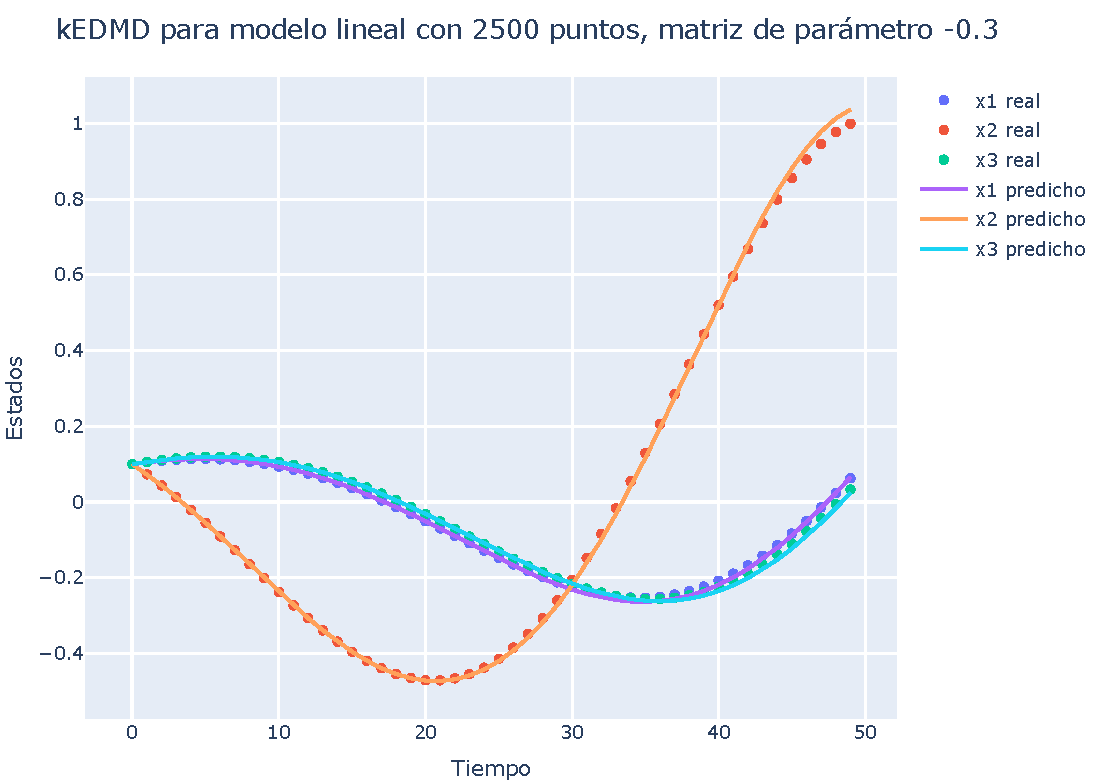
\includegraphics[width=\textwidth]{img/content/chapter3/Linear1.pdf}
        \caption{Imagen 1}
        \label{fig:image1}
    \end{subfigure}
    \hfill
    \begin{subfigure}[b]{0.32\textwidth}
        \centering
        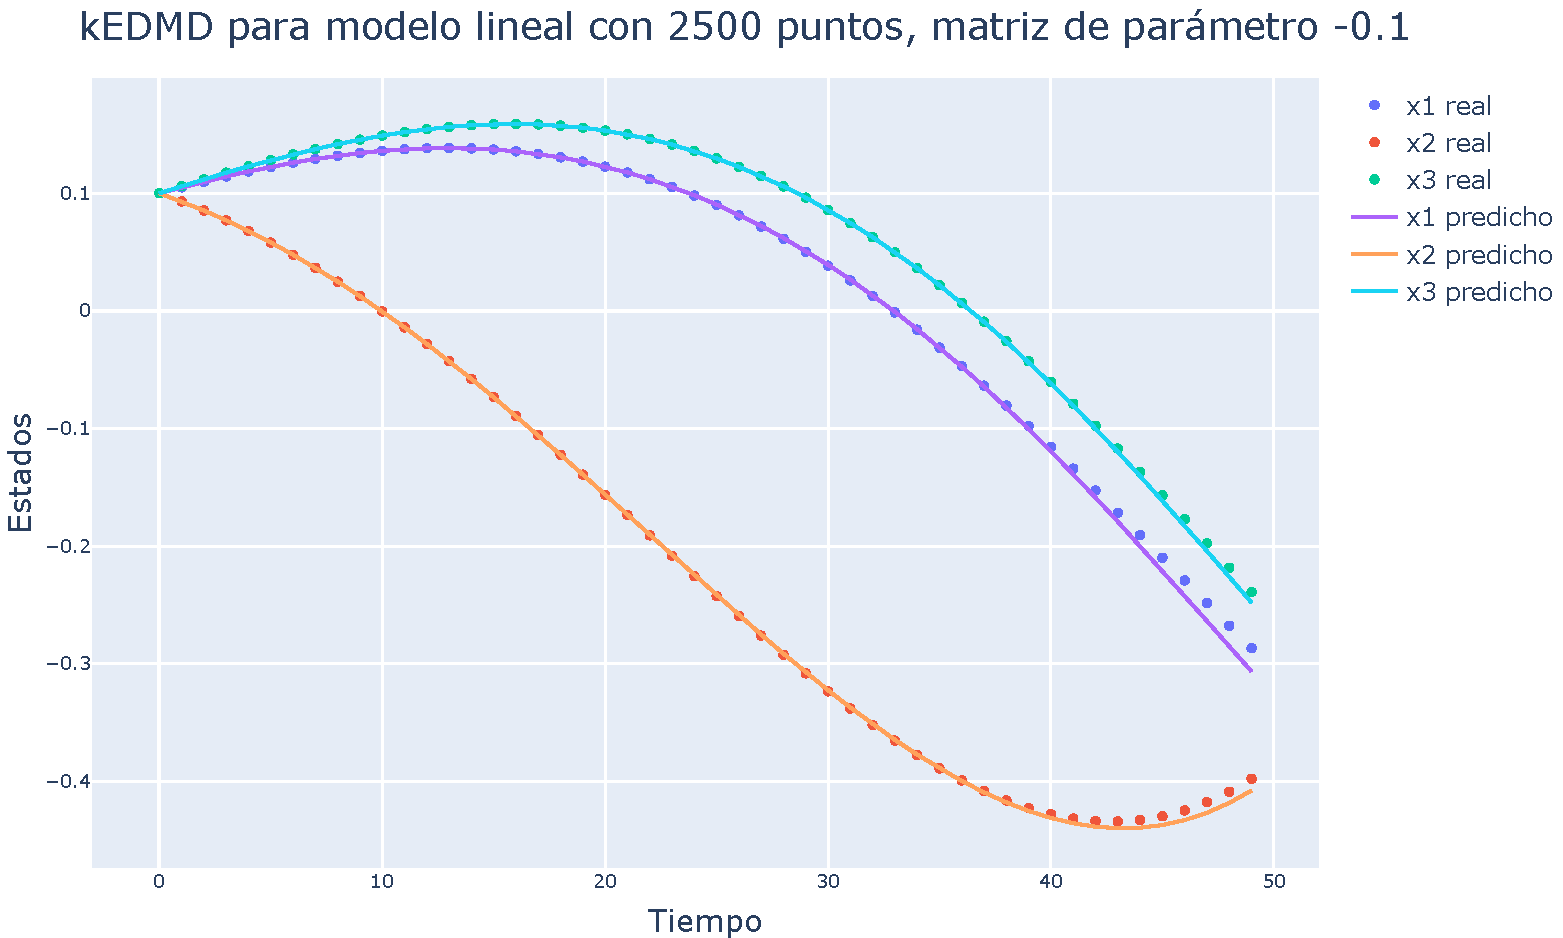
\includegraphics[width=\textwidth]{img/content/chapter3/Linear2.pdf}
        \caption{Imagen 2}
        \label{fig:image2}
    \end{subfigure}
    \hfill
    \begin{subfigure}[b]{0.32\textwidth}
        \centering
        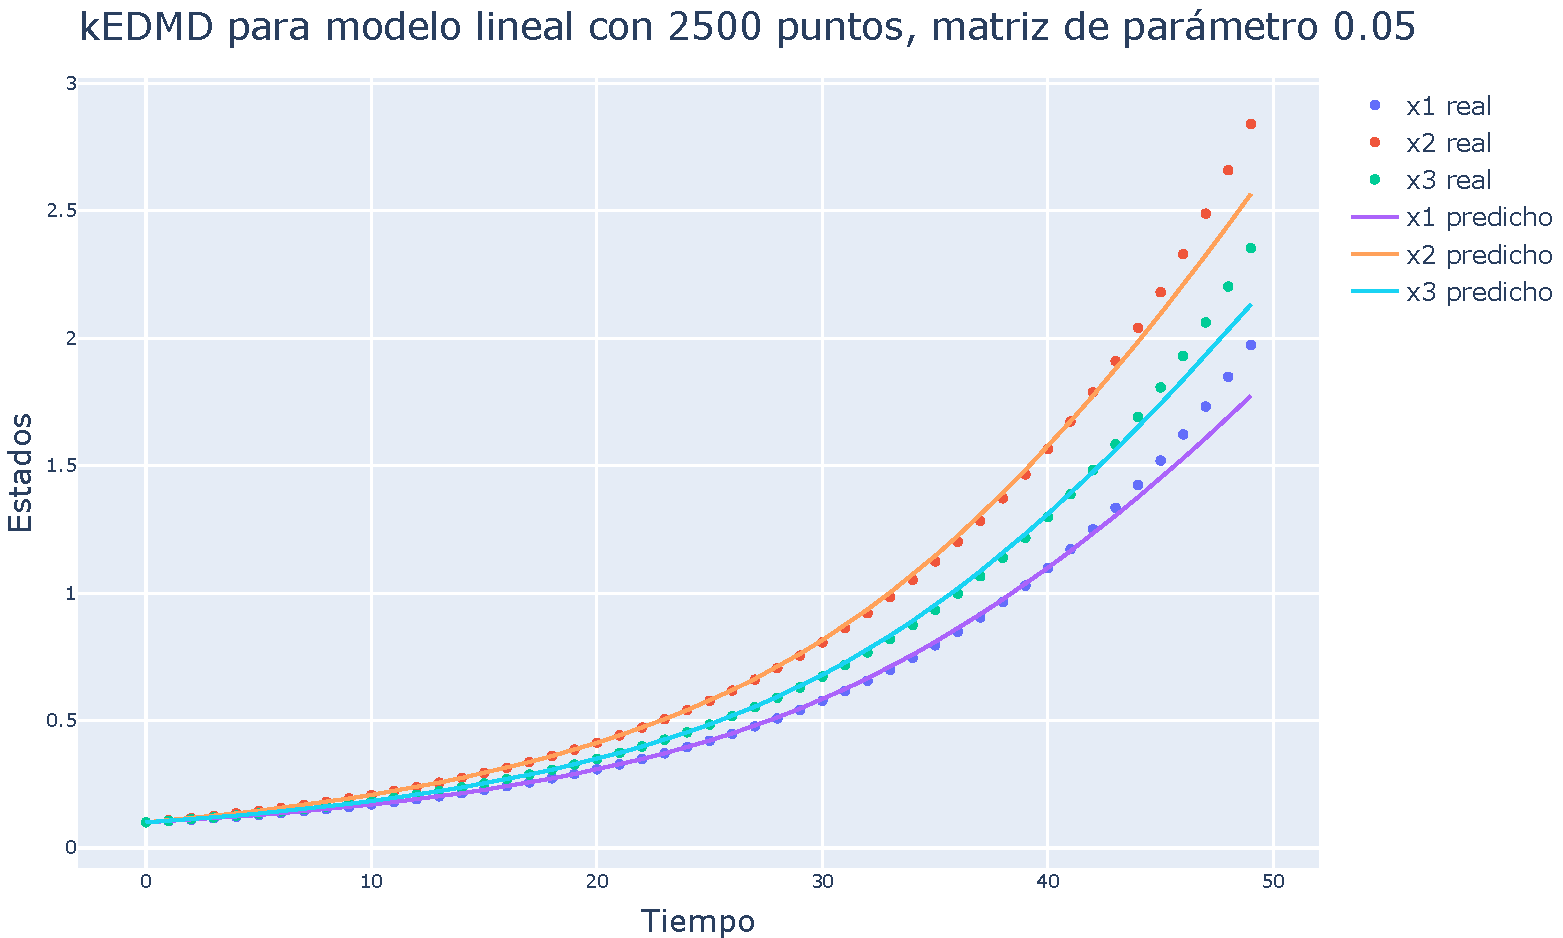
\includegraphics[width=\textwidth]{img/content/chapter3/Linear3.pdf}
        \caption{Imagen 3}
        \label{fig:image3}
    \end{subfigure}
    \caption{Tres imágenes en una línea}
    \label{fig:three_images}
\end{figure}